\endinput
% \begin{figure}[h!] 
	\centering
	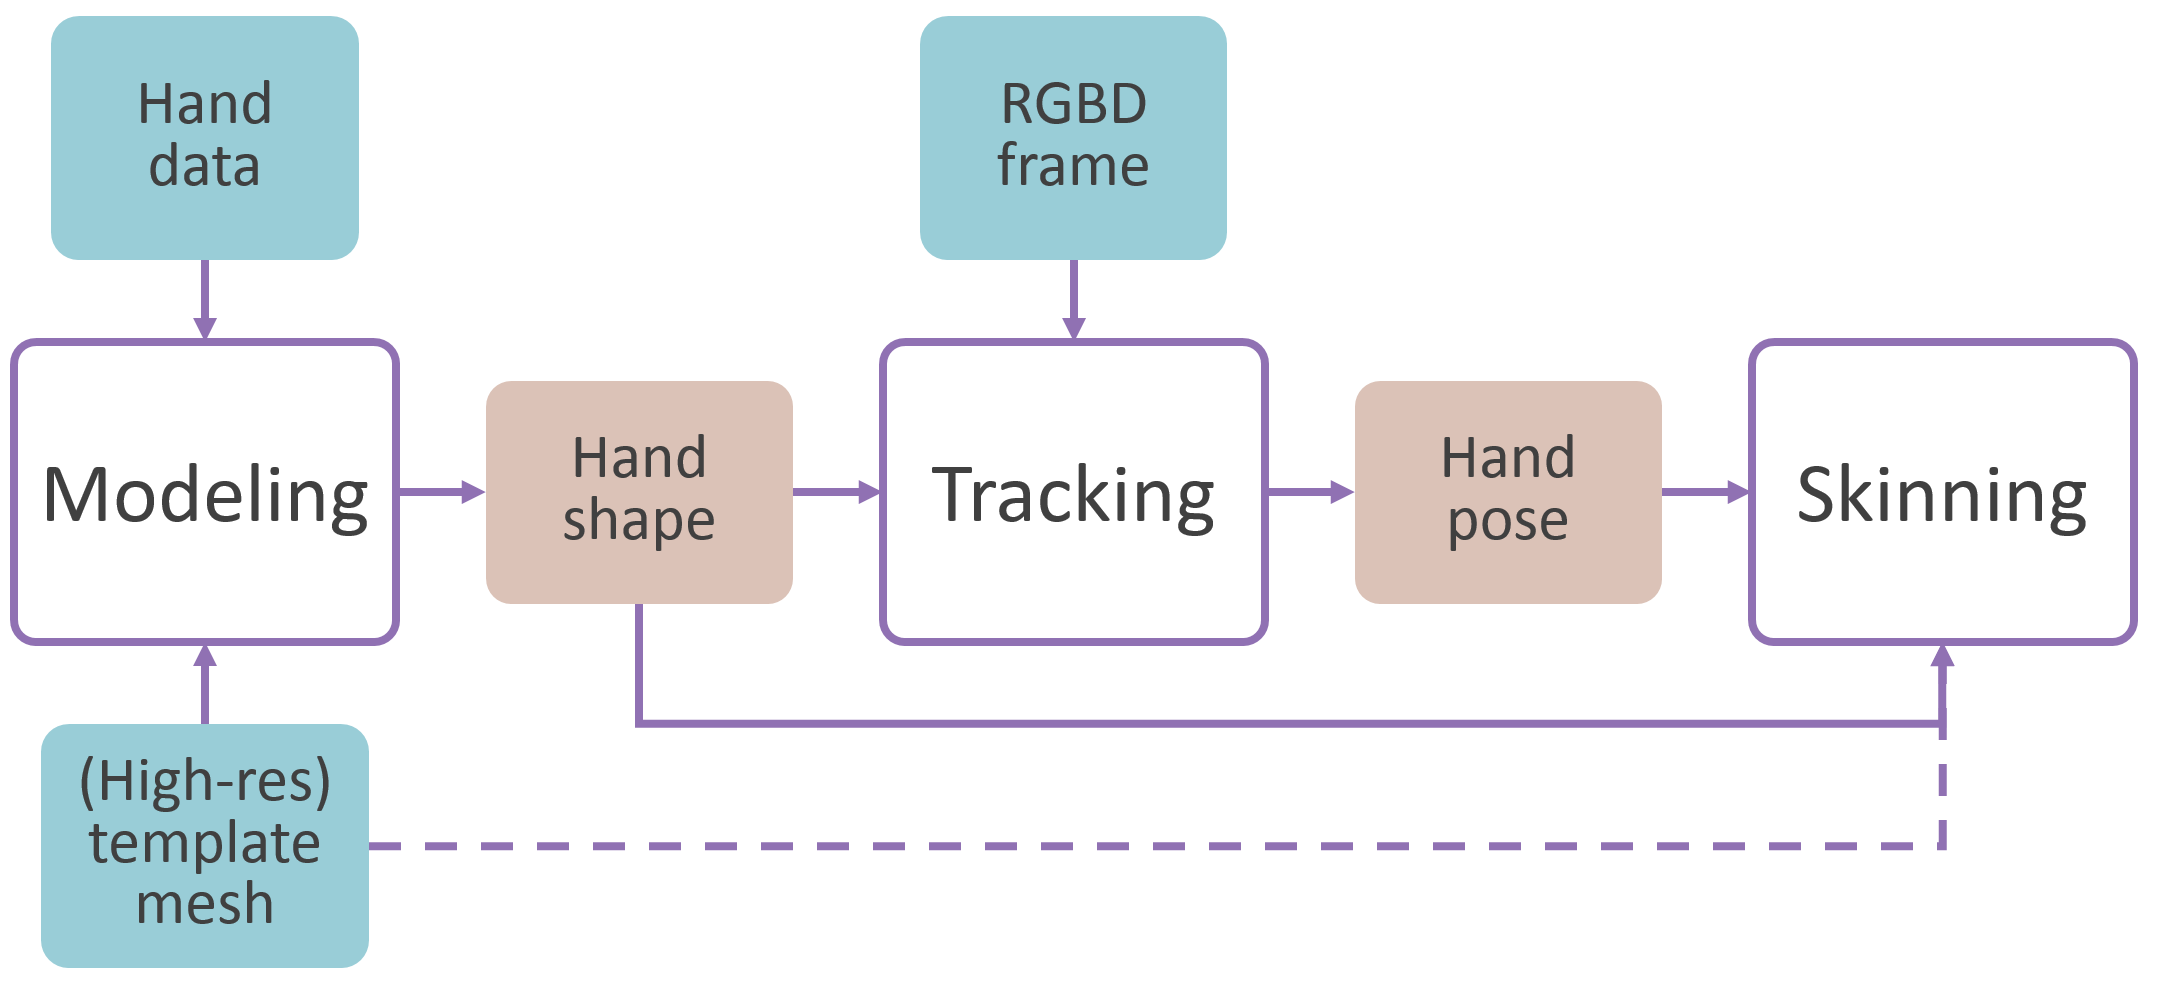
\includegraphics[width=0.5\textwidth]{fig/generic_pipeline}
	\caption{Generic pipeline for hand tracking. The input data that does not depend on the internal hand model representation is shown in blue, the representation-dependent components are shown in beige, and are listed in Table \ref{table:representation_dependent_components} for different representations.}
	\label{fig:generic_pipeline}
\end{figure} %<<< TO REMOVE!

% \paragraph{Rigidity - OLD}
% \begin{DRAFT}
% We encode this requirement by requiring each edge $\edge_k$ in each posed skeleton $\skeleton_n$ to be a rotation of rotation $R_{k}$ of its rest-pose configuration~$\bar\edge_k$:
% \begin{equation}
% E_{\text{rigid}} = \sum_{\edge_k \in \skeleton_n} \| \edge_k  - R_{k}{\bar\edge_k} \|_2^2
% \label{eq:rigidity}
% \end{equation}
% Note that only a subset of the edges of our control skeleton, as illustrated in \Figure{topology}, are required to satisfy this rigidity requirement. At the cost of introducing auxiliary variables $R_{i}$, this energy becomes independent from pose $\parposes$ and posture $\parposture$ angles.
% \end{DRAFT}
%

% pose and posture are optimized jointly by fixing the geometry of the template and aligning multiple instances to each frame. The kinematic chain is adjusted by refining the rest-pose transformations $\mathbf{\bar{T}}_k$; note only the rotational degrees of freedom of $\mathbf{\bar{T}}_k$ are optimized for, as frame translations are inferred from $\skeleton$.

% The first reason is that we want ensure that the resulting hand model will be able to assume all the poses that a real hand can, or at least the subset of poses for which we have the point clouds.
% The second reason is that the artifacts present in some input point clouds might be compensated by the others, so it is possible to accumulate information this way.
% For fitting we use the same optimization framework as for tracking (in a hope to extend it to fitting \& tracking real time system).
% The main difference is that instead of the joint angles $\theta$, the hand model is parametrized by convolution surface centers locations and radii $[c , r]$.
% \begin{equation*}
% \sigma =\underset{\sigma}{\operatorname{argmin}} \; E_\text{d2m} + E_\text{m2d} + E_\text{rigid} + E_\text{valid}
% \end{equation*}
% \subsection{Optimization}

% \paragraph{Synchronizing rotations energy}
% \AT{This is now obsolete, as we encode common rotation frames for nodes of the kinematic chain} This energy ensures that initial rotations are similar for all the poses. The common initial rotations are computed as described in the section ``Initial Rotations''. The energy minimizes the distance between the current centers and the centers locations with common initial rotations. This energy is very important, because it constraints fingers motion in meaningful way. In the absence of this energy each joint bends in arbitrary direction.

% The first attempt was to make the model-data energy also the same as in Htrack. But probably due to more non-linear gradients that expression was giving unstable optimization, because it was involving a projection operator. So, the model-data energy is replaced by a similar energy, but in 3D space. \Anastasia{Maybe we could just say that it is exactly the same?}.
% The model-data correspondences are also computed by rendering the model and the data, identifying the model points that are outside of the data silhouette and finding the closest data points in 2D using a distance transform. Afterwards for each 2D correspondence pair $\{m_{2D}, p_{2D}$\}, the original 3D points $\{m, p\}$ are looked up. We minimize the distance between $m$ and $p$ in the direction orthogonal to the camera ray that goes through $p$.
% \begin{figure}[h!]
\centering
\begin{overpic} 
[width=\linewidth]
{fig/optimization/item.pdf}
\end{overpic}
\caption{{Model-data energy}}
\label{fig:onecol}
\end{figure}
% \begin{equation*}
% E_\text{model-data} = \underset{m\in M}\sum n^T(p - m(\sigma))
% \end{equation*}

% This energy ensures that pills do not degenerate into spheres and wedges do not degenerate into pills. A pill becomes degenerate if one of the spheres is completely inside of another sphere. A wedge becomes degenerate if a sphere is completely inside of the tangent cone of two other spheres. The energy switches on if a pill or a wedge is within a threshold of becoming degenerate and pushes the optimization away.

% 
%In this section explain how we build our template model in an off-line preprocess and then discuss how this template can be adjusted to a specific user from RGBD sensor data. \AT{this makes it sounds like a two-steps approach... but it's really not? Also see below.}
%
%\subsection{Template construction}
%\begin{DRAFT}
%To obtain an accurate representation of hand geometry in different articulations, we scan a hand by taking on the order of ?? high-resolution photographs from different viewpoints for ?? different poses. From these images we compute dense point clouds for each pose using \emph{Agisoft Photoscan}.
%We manually specified the topology of our convolution surface depicted in Figure~\ref{fig:topology}. Then we optimize for the positions and radii, using manually specified initial values.
%\end{DRAFT}
%\AT{I am very confused about this ``template construction'' phase. As you can see in \Figure{calibration} there is not much to construct!}
%
%
%
%\subsection{User calibration} 

% In the accompanying video \todo{[00:00]}, we show how incorrect initialization of $\mathbf{\bar{T}}$ can be highly detrimental to tracking quality. For this reason,
% While for most articulations such an approximation is somewhat acceptable, it is particularly challenging to select the correct reference frame for the thumb articulation.
% However, this is not sufficient, as most tracking systems, including the one we build upon, parameterize a pose through the specification of a kinematic chain.
% An an example, transformations for the index finger are parameterized so to result in \todo{flexion} (resp. \todo{abduction}) as a rotation around the local $x$ (resp. $y$) axis.
% \AT{We should write $\restcenters$ as the positions at rest, while $\posedcenters$ as the set of posed convolution models.}

% \AT{I am very confused about what you wrote below, it doesn't look like an optimization problem at all... so in ``Chain Optimization'' I simply formalized what I had hand-written in the past -- please let me know if everything is clear!!.}
%
% \begin{DRAFT}
% To compute initial rotations we formulate an optimization problem for all the input hand poses. Denote the set of model centers in pose $i$ as $C_i = \{c_1^i, ... c_{|C_i| }^i\}$. As a preprocessing step we compute a rigid rotation between the rigid palm centers (the centers that are not articulated or elastic) and rotate all the poses to the same position, such that base centers of their fingers match together.
%
% The initial rotation is computed separately for each finger, so let us just discuss one finger. We minimize the norm of the difference between the centers of the finger at the current $i$ pose $\{c_1^i, c_2^i, c_3^i \}$ and the positions of the centers posed using the same initial rotations across all poses $\{\hat{c}_1^i, \hat{c}_2^i, \hat{c}_3^i \}$. Here $c_1^i$ stands for the base of the second phalange, $c_2^i$ stands for the base of the third phalange, and $c_3^i$ the end of the third phalange.
%
% Denote the initial rotations of the first, second and third phalanges as $I_1$, $I_2$ and $I_3$. We parametrize initial rotations of a finger by 5 values $\alpha = \{\alpha_1, ..., \alpha_5\}$, such that $I_1 = R_z(\alpha_3) R_y(\alpha_2) R_x(\alpha_1).$ \Anastasia{it is in reversed order to much the way the rotations are applied in Htrack, probably this should not  go to the paper} $I_2 = R_z(\alpha_4)$ and $I_3 = R_z(\alpha_5)$, where $R_x$, $R_y$ and $R_z$ are rotations around axis $X$ (side), $Y$ (up) and $Z$(front). We choose not to allow initial rotations around $X$ and $Y$ for the second and third segment partially to decrease the smallest number of required hand poses, partially because it seems that this rotations do not exist in real hand.
%
% Denote the rotations given by the values of the joint angles for the pose $i$ for the phalanges as $J_1^i$, $J_2^i$ and $J_3^i$.
% \begin{equation*}
% J_1^i = R_x(\theta_2^i) R_z(\theta_1^i),
% J_2^i = R_x(\theta_3^i),
% J_3^i =  R_x(\theta_4^i),
% \end{equation*}
% where $\theta_1^i$ and $\theta_2^i$ are abduction and flexion of the first phalange and $\theta_3^i$ and $\theta_4^i$ are flexions of the second and third phalanges at the pose $i$.
% The positions of the centers posed with the same initial transformations are computed as following:
% \begin{align*}
% & \hat{c}_1^i =  t_1 + I_1   J_1^i    l_1  u, \\
% & \hat{c}_2^i = t_1 + I_1    J_1^i   (t_2 + I_2  J_2^i  l_2  u), \\
% &\hat{c}_3^i =  t_1 + I_1    J_1^i   (t2 +  I_2   J_2^i  (t_3 + I_3  J_3^i  l_3 u)),
% \end{align*}
% where $t_1$, $t_2$, $t_3$ and $l_1$, $l_2$, $l_3$ are the translations and length of the bases of the phalanges 1, 2 and 3. They are computed from the input locations of the centers are constants; $u$ is a vector along the axis $Y$ (up).
% \end{DRAFT}

% The overwhelming majority of hand  tracking systems uses joint angles as an optimization variable. Given the vector of joint angles $\theta$, one also needs to know the initial rotations of the fingers with respect to the palm to be able to pose the model. The precise tracking is impossible without having the correct initial rotations, because the joints at the base of fingers cannot rotate around their axis, thus initial rotations constrain the possible poses that a hand model can assume.
% The initial rotations of the fingers can be guessed approximately because the are close to identity, but with the thumb it is much more difficult. \Anastasia{To prove this, I could alter the rotations in our system and show that tracking gets worse.}

The triangles mesh representation can approximate the hand to a high precision. However, it is not trivial to specify the model parts that are rigid and should be kept the same shape between the poses. This results in overfitting to local skin deformations. 

However, in most consumer applications hand tracking is just a single components of a bigger pipeline (Figure \ref{fig:generic_pipeline}). Before tracking, a suitable hand model is obtained. Once the hand pose parameters are found, the tracking result is displayed by skinning the model. Both modeling and skinning tasks are not trivial.

\begin{figure}[h!] 
\centering
\hspace{-2em}
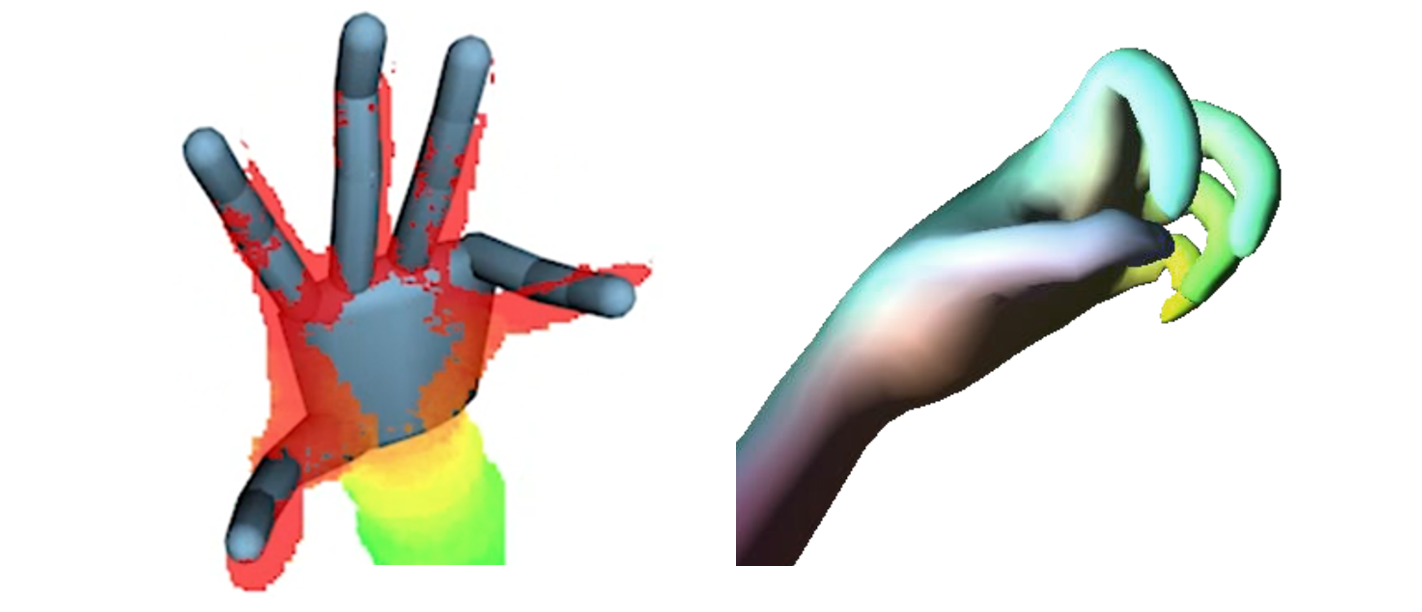
\includegraphics[width=0.5\textwidth]{fig/coarse_hand_model_and_lbs}
\caption{}.
\label{fig:coarse_hand_model_and_lbs}
\end{figure}

Especially if the hand model does not reflect all the degrees of freedom of a hand (Figure \ref{fig:coarse_hand_model_and_lbs}, left).

Each stage of the pipeline requires a hand model. There is several different hand model representations suggested by previous authors (see Figure \ref{fig:hand_model_representations}). Each representation is well suited for one of the stages, since it was used for the task on the first place. We argue that each representation also has weaknesses, which is why there exists a set of alternatives.

%--- OLD CONVOLUTION SURFACES TEXT
We suggest to use convolution surfaces representation of the hand model. Convolution surface is an implicit surface which is described by a control skeleton. The skeleton may consist of points, edges or polygons \cite{bloomenthal1991convolution}. In each vertex of the skeleton we define a radius. The radius in intermediate points is a linear combination of the radii at the neighboring vertices. Given the topology of the underlying skeleton, the model can be represented with convolution surface up to high precision \textcolor{mygray}{(find some theoretical estimates).} Next we present the arguments why convolution surfaces representation is suitable for all the stages of the pipeline.

%--- Linear blend skinning
The hand skinning quality is obviously important for digital avatars applications. The simple skinning approaches like linear blend skinning may generate implausible results.

\begin{table}[!ht] 
	\centering
	\begin{tabular}{|p{2.5cm}|p{2.5cm}|p{2.5cm}|}
	\hline
 	& Hand pose  & Hand shape  \\
	\hline
	Triangular mesh with embedded skeleton, \cite{taylor2014user} & Vertices and bones positions & Vertices and bones positions	 \\
	\hline
	Cylinder model, \cite{tagliasacchi2015robust} & Cylinders size and transformations & Cylinders transformations	 \\
	\hline
	Convolution surfaces model & Positions and radii of control points & Positions of control points \\
	\hline
	\end{tabular}
	\vspace{1em}
	\caption{Comparison of different hand model representations}
	\label{table:representation_dependent_components}
\end{table}

\subsection{Convolution surfaces for model fitting}
The spheres and mixed cylinders/spheres hand model representations (Figure \ref{fig:hand_model_representations} a, b) are ubiquitous in hand tracking, because they are well suited for tracking tack per se (see next) and can be quickly to created manually. If a small number of  building blocks is used, the precision of the model is low, especially in the palm region. 


% In convolution surfaces correspondence computation takes place in four steps:
% \todo{If our convolution model would be composed of a single skeletal element, the computation of correspondences would be as visualized in~\Figure{corresp}.}

% \begin{figure}[b]
\centering
\begin{overpic} 
[width=\linewidth]
{fig/silhouette/item.png}
\end{overpic}
\caption{
% 
% 
(left) The silhouette of the model computed by projecting the model in the camera plane (\todo{fingers outline is computed separately, here an entire model outline is shown for illustration purposes}). (right) The silhouette curves, marked in pink, are re-projected in 3D. 
\AT{why in the image in the left it's only the image-space silhouette with a pink boundary, while on the right you can also find the silhouette in the interior?}
\Anastasia{As I mentioned, for illustration purposes, to show to the outline is always outside of the model. Probably it is a bad idea, I should just display the same outline as on the right, because that is what I actually compute.}
} 
\label{fig:silhouette}
\end{figure}

\begin{algorithm}
\caption{Correspondences computation}
\begin{algorithmic}[1]
    \For {$\text{each } p$}
    	 \State \text{compute model projection } $q_m$
    	 \State \text{replace or discard if $q_m$ is back-facing}
    	 \State \text{compute outline projection } $q_o$
         \State $q=(\|{p - q_m}\|_2^2 < \|{p - q_o}\|_2) ? q_m : q_o$
    \EndFor
\end{algorithmic}
\label{alg:correspondences}
\end{algorithm}

% \textbf{Computing model projection.}
% taking the minimum helps to get the projection on the model surface when the data point $p$ is inside of the model \AT{how? I am not sure I understand, please quickly sketch a figure!)}.

\textbf{Discarding or replacing back-facing projections.}
\begin{itemize}
	\item Convolution segment: the closest front-facing point is on the model outline, thus set the current point $q_m$ to $\infty$.
	\item Convolution triangle: the closest front-facing point is either on the model outline or on a front-facing face of the convolution triangle, thus replace $q_m$ by the closest front-facing face projection.
\end{itemize}

% For this computation we assume that projection is orthographic and that camera direction coincides with axis $Z$. We shift all the model spheres to have zero coordinate at axis $Z$ and compute an outline of the cross-section of the model with the $XY$ plane.
To obtain the 3D outline we shift the model spheres with attached 2D outline back to their original positions. The model outline is represented as a sequence of line and circle segments. To compute an outline projection $q_o$ we compute a projection on each element of the outline and select the closest to the data point $p$.

% We first shift all the model centers to have zero coordinate at the axis Z (which coincides with camera axis). We compute the cross-section of the model with XY plane. This cross-section consists of  circles and line segments (see \Figure{silhouette}, left).

% We traverse this graph starting from the upper left or any other point that is guaranteed to be on the outline. From every vertex we follow the edge with the next polar angle from the one that we came from (for the circle the polar angle is computed for a tangent at that point). This way  we always stay on the outline and never go inside of the cross-section.

% Now we need to find a set of circle segments and line segments that are on the outline of the cross-section.  This is done by computing intersection and tangency points of every circle with every other circle and every line segment. The resulting structure can be thought of as a graph with intersection and tangency points as vertices and circle and line segments as edges.
% We traverse this graph starting from the upper left or any other point that is guaranteed to be on the outline. From every vertex we follow the edge with the next polar angle from the one that we came from (for the circle the polar angle is computed for a tangent at that point). This way  we always stay on the outline and never go inside of the cross-section.

% Note that if a finger is in front of the palm, we still want to have its outline for the benefit of the correspondences that are back-facing to the finger. Therefore we separately compute the outline for the palm and for the fingers and merge them together afterwards. 

% The merging is done by removing the part of the finger outline that is inside of the palm outline and part of the palm outline that is inside of the finger outline. The fingers outline only modified if it is the outline of the base finger segment, because it is OK for the finger tip outline to be inside of the palm outline.